\section{Resultados}
Os resultados da execução de cada função mostra como o está o funcionamento do sua funcionalidades. 

\subsection{Amostra das execuções}

\subsubsection{Ping Flooder}
O flooder de pacotes Ping mostrou um bom funcionamento. No exemplo abaixo mostra uma rápida execução desse flooder onde os endereços de IP e MAC do alvo foram informados e o endereço MAC de origem usado foi o local, MAC da interface usada.
\begin{figure}[h]
    \centering
    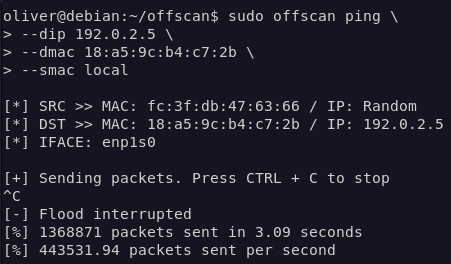
\includegraphics[width=0.45\textwidth]{fotos/ping.png}
    \caption{Execução do flooder de pacotes Ping}
\end{figure}


\subsubsection{TCP Flooder}
O flooder de pacotes TCP SYN também mostrou bom funcionamento. No exemplo abaixo mostra uma rápida execução desse flooder onde, além das informações usadas no exemplo anterior, a porta foi informada.
\begin{figure}[h]
    \centering
    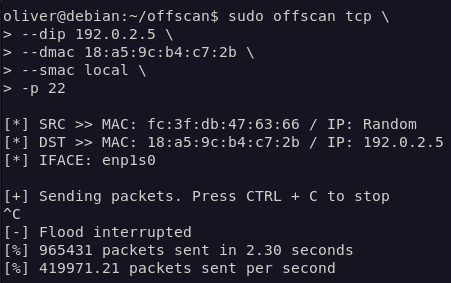
\includegraphics[width=0.45\textwidth]{fotos/tcp.png}
    \caption{Execução do flooder de pacotes TCP}
\end{figure}


\subsubsection{Ataque de desautenticação}
O ataque demonstrou ser eficaz em provocar a desassociação do cliente do ponto de acesso. O tempo de reação do dispositivo alvo fica entre 15 e 30 segundos.
\begin{figure}[h]
    \centering
    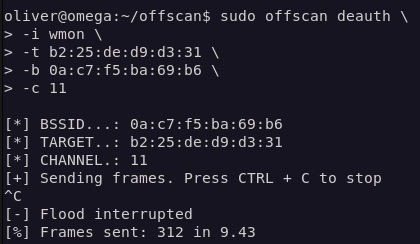
\includegraphics[width=0.45\textwidth]{fotos/deauth.png}
    \caption{Execução do mapeador de rede}
\end{figure}



\subsubsection{Mapeador de redes}
No exemplo abaixo, apenas o comando para mapear a rede foi informado. Com isso, a interface padrão é usada e a partir do IP e da mascara da rede, todos os IPs da rede são calculados para serem escaneados.
\begin{figure}[h]
    \centering
    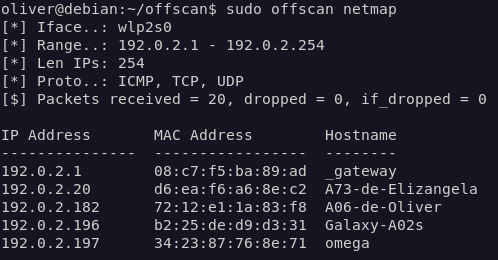
\includegraphics[width=0.46\textwidth]{fotos/netmap.png}
    \caption{Execução do mapeador de rede}
\end{figure}


\subsubsection{Informações de Rede e Interface}
No exemplo abaixo o comando \texttt{info} foi executado. Ele mostra informações da interface que foi escolhida e da rede ao qual está conectada, se estiver.
\begin{figure}[h]
    \centering
    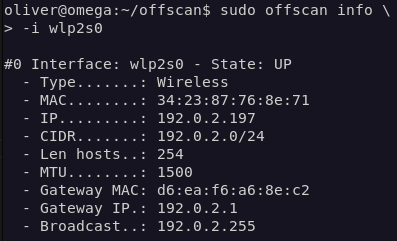
\includegraphics[width=0.46\textwidth]{fotos/info.png}
    \caption{Execução do comando \texttt{info}}
\end{figure}


\subsubsection{scanner de portas}
Na amostra abaixo, o scanner varreu as portas do gateway. Veja que ele apenas mostra qual a porta aberta, não o serviço.
\begin{figure}[h]
    \centering
    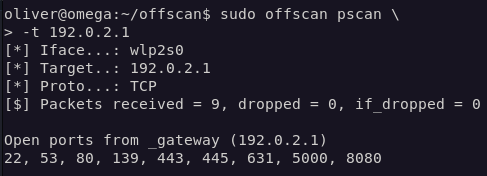
\includegraphics[width=0.46\textwidth]{fotos/pscan.png}
    \caption{Execução do scanner de portas}
\end{figure}


\subsubsection{Mapeador de redes Wi-Fi}
No exemplo desse comando foram alterados o nome da rede (SSID) e parte do BSSID de cada rede para preservar a privacidade. A imagem abaixo mostra como o comando mostra as informações que pegou de cada rede Wi-Fi.
\begin{figure}[h]
    \centering
    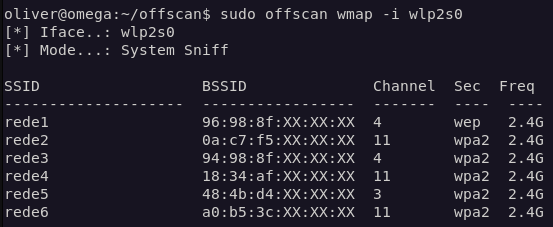
\includegraphics[width=0.46\textwidth]{fotos/wmap.png}
    \caption{Execução do mapeador de redes Wi-Fi}
\end{figure}


\subsubsection{Flooder de beacons}
O flooder de beacons se mostrou muito eficiente como mostra a imagem abaixo. Nela, é possível ver algumas das muitas redes inexistentes que os beacons transmitiram.
\begin{figure}[h]
    \centering
    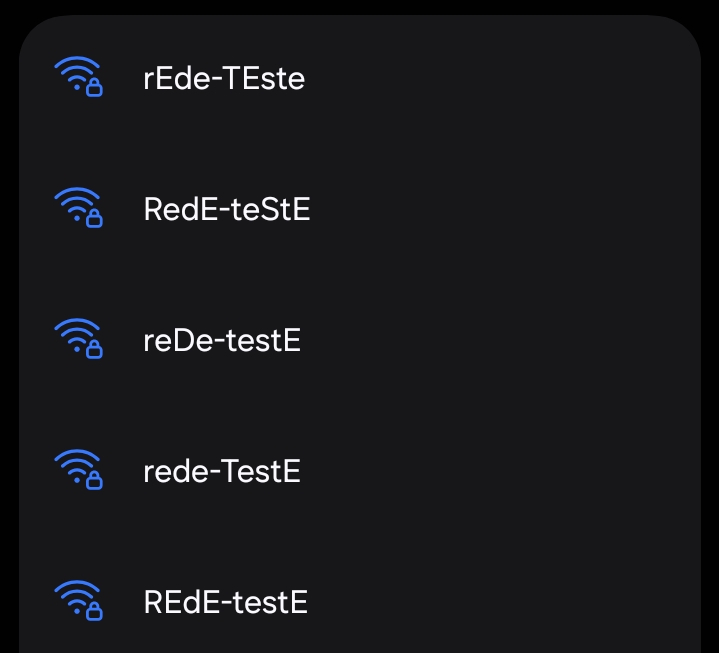
\includegraphics[width=0.46\textwidth]{fotos/beacon.jpg}
    \caption{Execução do flooder de beacons}
\end{figure}


\subsection{Análise dos resultados}
Com base nas execuções, observou-se que: 

\begin{itemize}
    \item \textbf{Flooder TCP e ICMP}: Ambas as funcionalidades alcançaram taxas médias de envio superior a 400.000 pacotes por segundo em redes cabeadas.
    
    \item \textbf{Flooder de beacons}: A taxa de envio foi limitada intencionalmente para evitar a saturação do espectro e permitir a visualização clara das redes falsas. Apesar dessa limitação, a funcionalidade mostrou-se eficaz, com múltiplos dispositivos detectando as redes falsas criadas.
    
    \item \textbf{Ataque de desautenticação}: O tempo médio para desconexão dos dispositivos-alvo variou entre 15 e 30 segundos. Notou-se que, em alguns casos, foi necessário reiniciar o envio dos quadros para manter a desconexão, indicando uma possível reassociação automática do cliente.

    \item \textbf{Mapeamento Wi-Fi}: A ferramenta obteve sucesso em detectar todas as redes sem fio dentro do alcance do dispositivo, tanto no modo \texttt{SysSniff} (através da API do kernel) quanto no modo \texttt{MonitorSniff} (interface em modo monitor).
    
    \item \textbf{Mapeador de redes}: Demonstrou alta eficácia na descoberta de hosts ativos, identificando corretamente dispositivos conectados na rede através de múltiplos protocolos (ICMP, TCP, UDP).
    
    \item \textbf{scanner de portas}: Mostrou-se eficiente na identificação de portas abertas, tanto com a técnica SYN (TCP) quanto com payloads específicos (UDP). A taxa de falsos positivos foi baixa, e o desempenho foi satisfatório para varreduras em intervalos de portas comuns.
\end{itemize}